\documentclass[8pt]{extarticle}
\usepackage{fancyhdr}
\usepackage{multicol}
\usepackage[%
    %a5paper,
    papersize={5.5in,8.5in},
    margin=0.7in,
    top=0.75in,
    bottom=0.75in,
    %twoside
    ]{geometry}

\usepackage[svgnames]{xcolor}
\usepackage{graphicx}
\usepackage{fancyhdr}
\pagestyle{fancy}

\raggedcolumns
\setlength{\multicolsep}{0pt}
\setlength{\columnseprule}{1pt}

\makeatletter

\newif\if@mainmatter \@mainmattertrue

%% Borrowed from book.cls
\newcommand\frontmatter{%
    \cleardoublepage
  \@mainmatterfalse
  \pagenumbering{roman}}
\newcommand\mainmatter{%
    \cleardoublepage
  \@mainmattertrue
  \pagenumbering{arabic}}
\makeatother

%% Vary the colors at will

\definecolor{vegancolor}{rgb}{0,0.5,0.2}
\definecolor{veggiecolor}{rgb}{0.91,0.41,0.17}
\definecolor{headercolor}{rgb}{0.5,0.5,0.5}
\definecolor{quantitycolor}{rgb}{0.5,0.5,0.5}

%--------------------------------------------------------------------------------------------------------
% Your "recipes.sty" package starts here:
%% Thanks to alephzero for the excellent start:

\newcommand{\recipe}[2][]{%
    \newpage
    \lhead{}%
    \chead{}%
    \rhead{}%
    \lfoot{}%
    \rfoot{}%
    \section{#2}%
    \if###1##%
    \else
        \begin{center}
            \parbox{0.75\linewidth}{\raggedright\itshape#1}%
        \end{center}
    \fi
}
\newcommand{\prepAndCookTime}[2]{%
	\fancyhead[C]{\footnotesize\color{headercolor}Prep Time: $\,$#1 \\ Cook Time: #2}}
\newcommand{\vegetarianAndServings}[1]{%
     \fancyhead[R]{\footnotesize\color{veggiecolor}\textmd{Vegetarian} \\ \footnotesize\color{headercolor}
     	#1 servings}}
\newcommand{\veganAndServings}[1]{%
	 \fancyhead[R]{\footnotesize\color{vegancolor}\textmd{Vegan} \\ \footnotesize\color{headercolor}
	 	#1 servings}}
\newcommand{\cuisineAndTotalTime}[2]{%
     \fancyhead[L]{\footnotesize\color{headercolor}\textmd{Cuisine: $\quad\,\,$ #1 \\ Total Time: #2}}}
% Color the quantities
\newcommand{\quantities}[1]{\textcolor{quantitycolor}{#1}}

\newcommand{\temp}[1]{%
    $#1^\circ$C}
%% Optional argument is the width of the graphic, default = 1in
\newcommand{\showit}[3][1in]{%
    \begin{center}
        \bigskip
            \includegraphics[width=#1]{#2}%
            \par
            \medskip
            \emph{#3}
            \par
        \end{center}%
    }

%% Optional argument for a  heading within the ingredients section
\newcommand{\ingredients}[1][]{%
    \if###1##%
        {\color{SteelBlue!80!MidnightBlue}\Large\textsc{Ingredients}}%
    \else
        \emph{#1}%
    \fi
}

%% Use \obeylines to minimize markup
\newenvironment{ingreds}{%
    \parindent0pt
    \noindent
    \ingredients
    \par
    \smallskip
    \begin{multicols}{2}
    \leftskip1em
    \rightskip0pt plus 3em
    \parskip=0.0em
    \obeylines
    \everypar={\hangindent2em}
}{%
    \end{multicols}%
    \medskip
}

\newcounter{stepnum}

%% Optional argument for an italicized pre-step
%% Also use obeylines to minimize markup here as well
\newenvironment{method}[1][]{%
    \setcounter{stepnum}{0}
    \noindent
    {\color{SteelBlue!80!MidnightBlue}\Large\textsc{Instructions}}%
    \par
    \smallskip
    \if###1##%
    \else
        \noindent
        \emph{#1}
        \par
    \fi
    \begingroup
    \parindent0pt
    \parskip0.25em
        \leftskip2em
    \everypar={\llap{\stepcounter{stepnum}\hbox to2em{\thestepnum.\hfill}}}
}{%
    \par
    \endgroup}

\pagestyle{fancy}
% End of "recipes.sty"

%--------------------------------------------------------------------------------------------------------
\begin{document}

\frontmatter
\tableofcontents

\mainmatter

%--------------------------------------------------------------------------------------------------------
\recipe[]{Coconut Curried Kale and Sweet Potato}
\prepAndCookTime{25 m}{40 m}
\veganAndServings{4}
\cuisineAndTotalTime{Indian}{1 h 5 m}
\begin{ingreds}
     \quantities{3 tbsp} extra-virgin olive oil
     \quantities{1} onion (slices)
     \quantities{2 pounds} sweet potato or butternut squash (cubes)
     \quantities{5 cloves} garlic (pressed or minced)
     \quantities{2 tsp} ginger
     \quantities{1 tsp} curry powder
     \quantities{2 pounds} kale (stemmed \& chopped)
\columnbreak
     \quantities{1 cup} vegetable broth
     \quantities{1 can} full-fat coconut milk
	\quantities{1 tbsp} lime juice
	\quantities{1/3 cup} green pumpkin seeds
	salt
	black pepper
(optional) red pepper flakes
\ingredients[Serves with:]
     Basmati rice 
\end{ingreds}

\begin{center}
	\includegraphics[width=0.30\textwidth]{recipePictures/CoconutCurriedKaleAndSweetPotato}
\end{center}

\begin{method}%[Preheat the oven to Gas Mark 4, Electric \temp{180}, Fan \temp{160}.]
     Warm 2 tablespoons olive oil (in a Dutch oven) over medium heat until shimmering. Add onion and cook, stirring frequently, until softened ($\sim$ 5 minutes). Add sweet potato or squash, cover and cook, stirring occasionally, until the sweet potato is bright orange (or until the butternut is just beginning to brown), ($\sim$ 5 minutes). Transfer the mixture to a bowl for now.

     Add 1 tablespoon olive oil to the pot and raise the heat to medium-high. Add garlic, ginger and curry powder and cook, stirring constantly, until fragrant ($\sim$ 30 seconds). Add half of the kale and stir until it’s beginning to wilt ($\sim$ 1 minute). Stir in remaining greens, broth, all but 1/2 cup coconut milk and 1/2 teaspoon salt.
     
     Cover pot, reduce heat to medium low, and cook, stirring occasionally, until kale is wilted ($\sim$ 12-15 minutes). Pour in sweet potato or squash mixture, cover and continue to cook until kale and sweet potato or squash are tender ($\sim$10-20 minutes).
     
     Cook the rice.
     
     (optional) Meanwhile, toast the pepitas in a medium skillet over medium-low heat, stirring frequently, until they’re fragrant and making little popping noises ($\sim$ 3-5 minutes). Transfer to a bowl to cool.
     
     Once the kale and sweet potato/squash are tender, uncover the pot and increase heat to medium-high. Cook, stirring occasionally, until most of the liquid has evaporated and sauce has thickened ($\sim$ 2-5 minutes).
     
     Remove from heat and stir in the remaining coconut milk. Add the lime juice and season with salt, pepper and optional red pepper flakes, to taste. Divide rice into bowls, then top with kale mixture and a generous sprinkling of pepitas before serving.
\end{method}

%--------------------------------------------------------------------------------------------------------
\recipe[]{Egg-Tomato-Potato Afghani Omelette}
\prepAndCookTime{10 m}{10 m}
\vegetarianAndServings{2}
\cuisineAndTotalTime{Afghani}{20 m}
\begin{ingreds}
	\quantities{4 tbsp} olive oil
	\quantities{4} eggs
	\quantities{1} onion
	\quantities{1} potato
	\quantities{2} tomatoes
	\quantities{1/2 tbsp} tomato paste
	salt
	black pepper
	\ingredients[Serves with:]
	Rice 
	Bread
\end{ingreds}

\begin{center}
	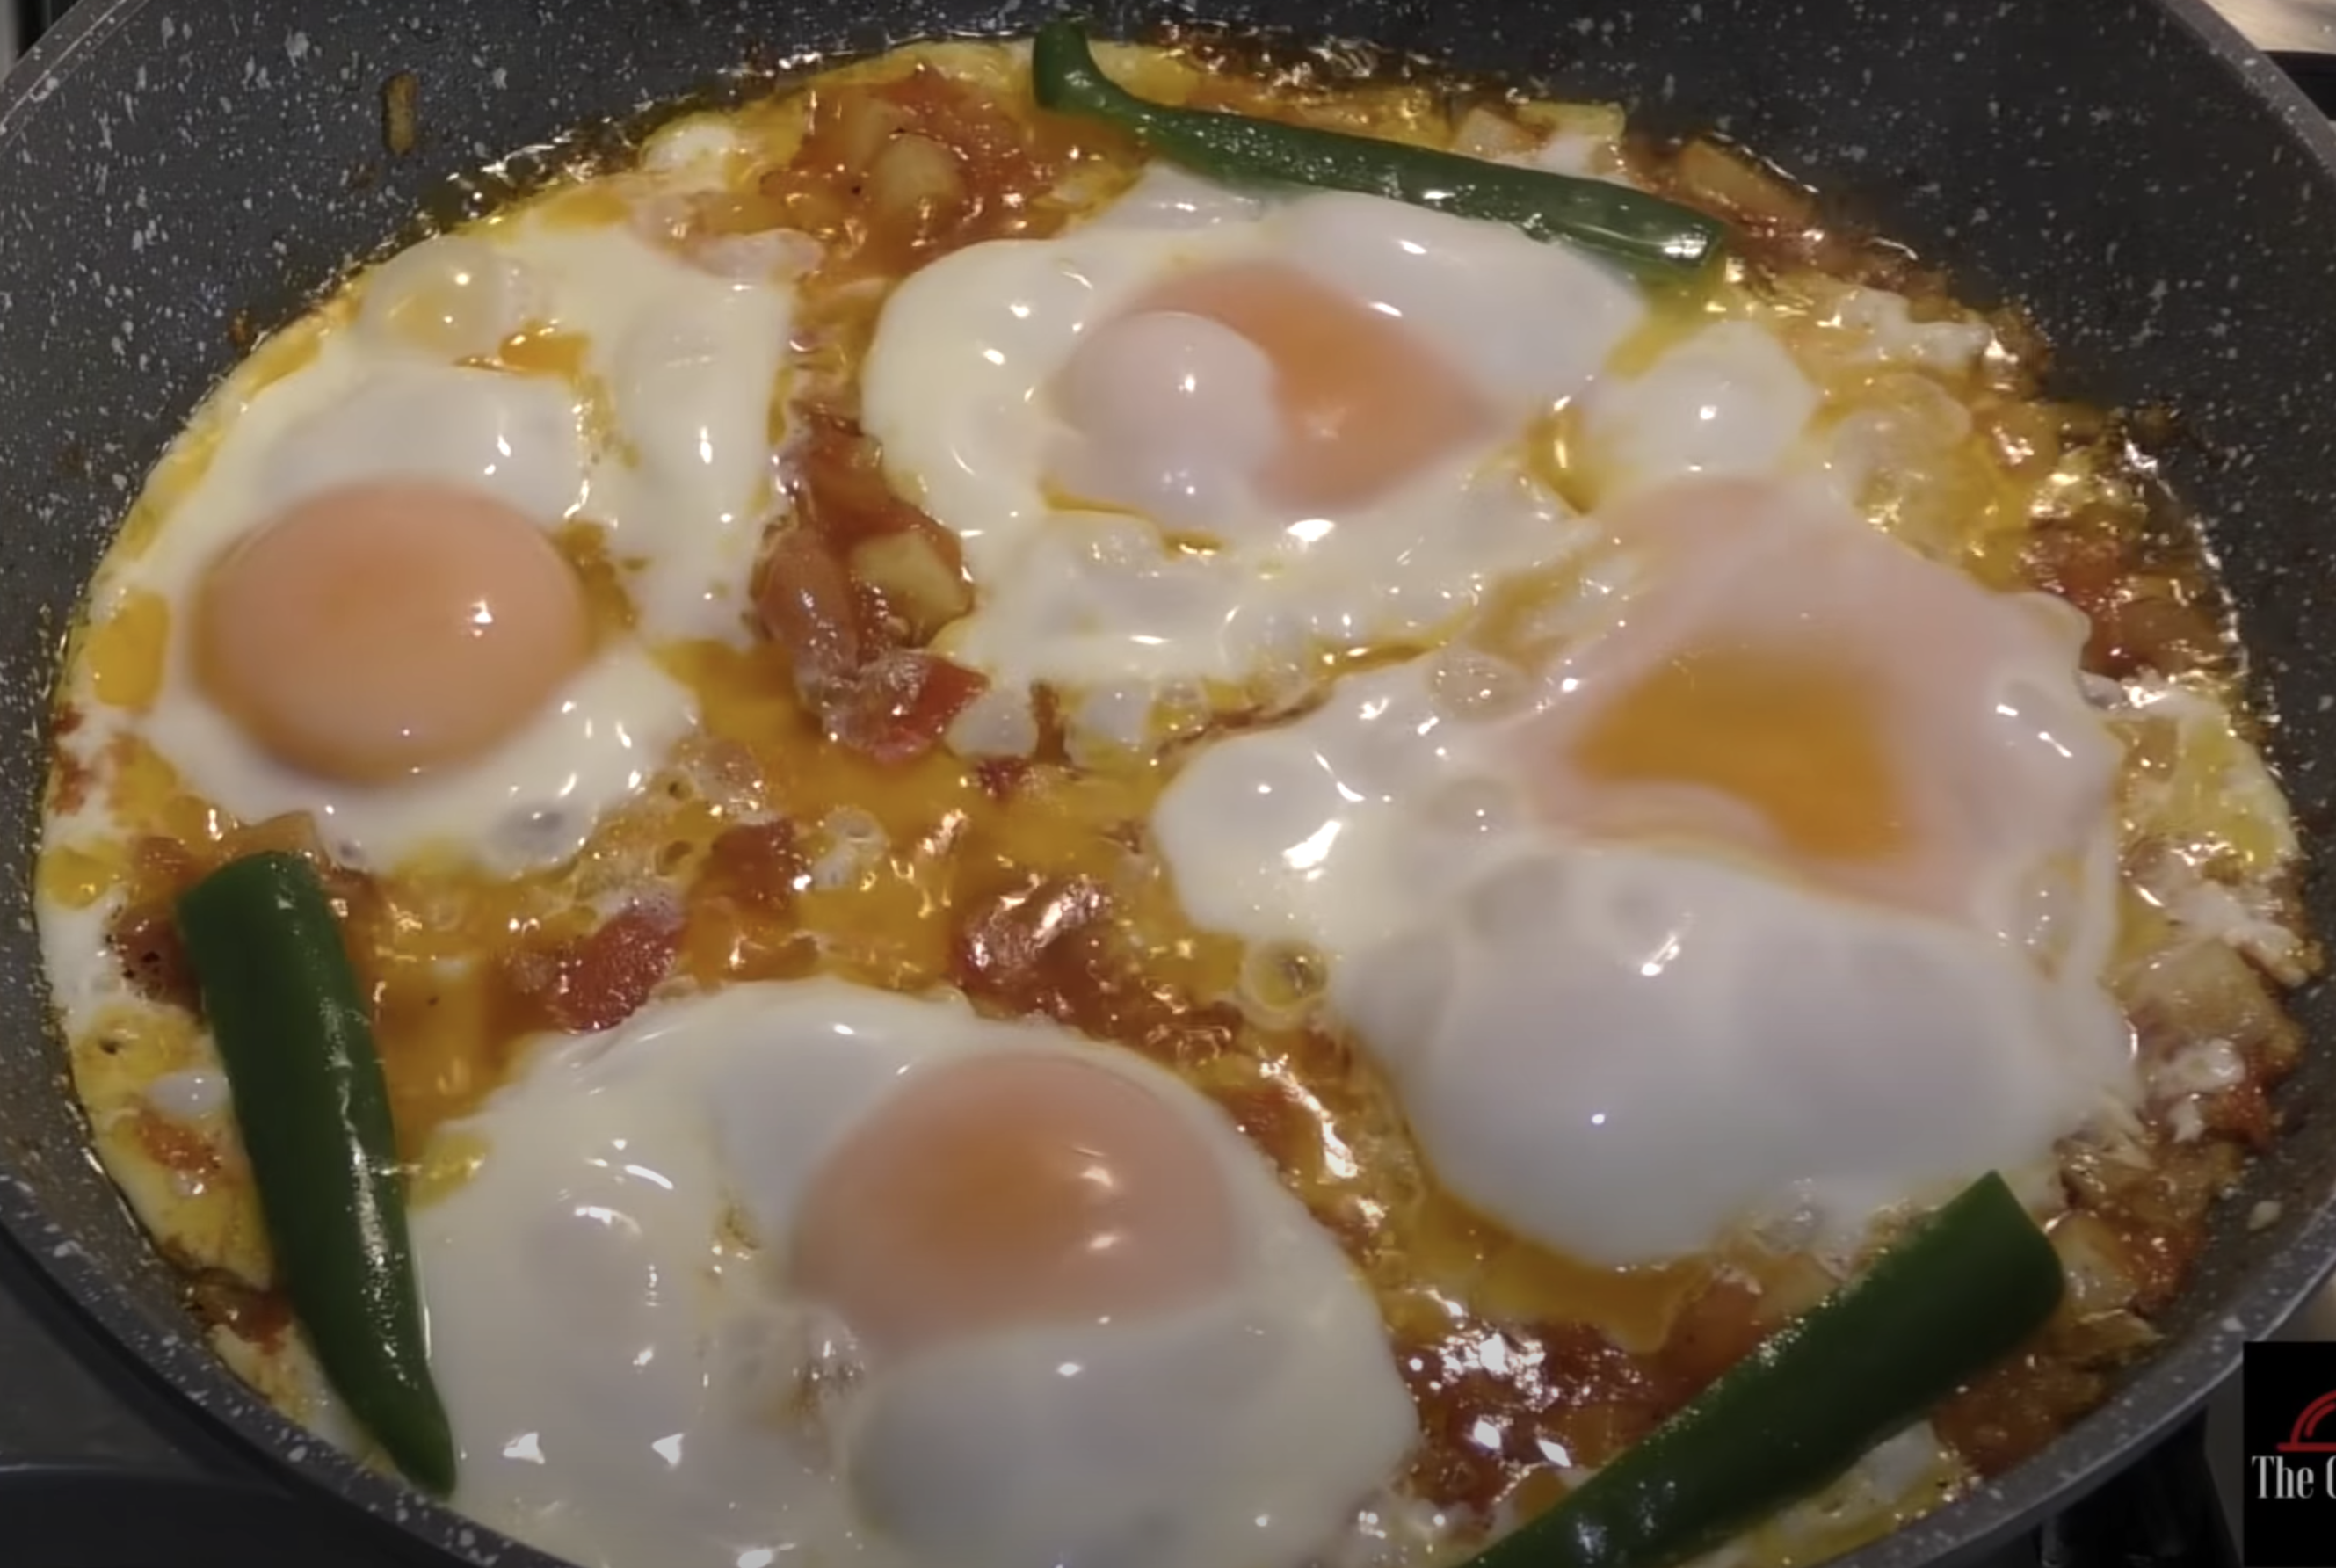
\includegraphics[width=0.30\textwidth]{recipePictures/EggTomatoPotatoAfghaniOmelette}
\end{center}

\begin{method}%[Preheat the oven to Gas Mark 4, Electric \temp{180}, Fan \temp{160}.]
	Heat up olive oil.
	
	Add the potatoes and cook for 4-5 minutes.
	
	Add the onion and cook for 2 minutes.
	
	Add salt and black pepper.
	
	Add tomatoes and cook until soft.
	
	(optional) Add tomato paste and cook for 1 minute.
	
	Add the eggs on top, cover and cook on medium flame for about 1 minute. (optional) Add fresh chilies on top
\end{method}

%--------------------------------------------------------------------------------------------------------
\recipe[]{Spicy Coconut Vegetable Stir Fry}
\prepAndCookTime{20 m}{15 m}
\veganAndServings{2}
\cuisineAndTotalTime{Asian}{35 m}
\begin{ingreds}
	\textsc{Sauce:}
	\quantities{1 can} full-fat coconut milk
	\quantities{1/4 cup} natural peanut butter
	\quantities{2 tbsp} sriracha
	\quantities{1 tsp} brown sugar
	\quantities{1 tbsp} soy sauce
	\quantities{1} lime
	\quantities{1 clove} garlic (minced)
	\quantities{1 tsp} fresh ginger (grated) 
	\phantom{.}
	\phantom{.}
	\textsc{Stir Fry:}
	coconut cooking oil
	\quantities{4-6 cups} mixed vegetables (carrots, brokkoli, pepper, green beans, onion)
	\ingredients[Serves with:]
	Basmati rice / Rice Noodles
	Tofu / Chicken / Shrimp / Tempeh
	peanuts (chopped)
	cilantro (chopped)
	lime (cutted into wedges)
\end{ingreds}

\begin{center}
	\includegraphics[width=0.30\textwidth]{recipePictures/SpicyCoconutVegetableStirFry}
\end{center}

\begin{method}%[Preheat the oven to Gas Mark 4, Electric \temp{180}, Fan \temp{160}.]
	In a medium bowl, mix together the coconut milk, peanut butter, sriracha, brown sugar, soy sauce, lime juice, garlic, and ginger. (If needed) Heat sauce gently. Taste sauce and adjust heat (sriracha), sweetness (brown sugar), tartness (lime juice).
	
	Heat up oil over medium. Add vegetables from hardest to softest. Stir fry accordingly until they begin to soften on the edges.
	
	Meanwhile, cook the rice.
	
	Pout sauce over, stir to combine \& allow sauce to heat through ($\sim$ 2 min). (If using tender green, like spinach, stir it into now until it has wilted)
\end{method}

{%%--------------------------------------------------------------------------------------------------------
\recipe[]{Instant Pot Pasta Mushroom Stronganoff}
\prepAndCookTime{15 m}{15 m}
\vegetarianAndServings{2}
\cuisineAndTotalTime{Russian}{30 m}
\begin{ingreds}
	\quantities{3 tbsp} olive oil
	\quantities{1/2} red onion
	\quantities{3 cloves} garlic
	\quantities{16 ounces} mushrooms
	\quantities{3/4 tsp} salt
	\quantities{1/2 tsp} pepper
	\quantities{1/4 cup} white wine
	\quantities{2 cups} veggie broth
	\quantities{1-2 tbsp} mustard
	\quantities{1 heaping tbsp} flour
	\quantities{8 ounces} uncooked pasta 
	\ingredients[Stir in after cooking:]
	\quantities{3/4 cup} cour cream
\end{ingreds}

\begin{center}
	\includegraphics[width=0.30\textwidth]{recipePictures/InstantPotPastaMushroomStronganoff}
\end{center}

\begin{method}%[Preheat the oven to Gas Mark 4, Electric \temp{180}, Fan \temp{160}.]
	Boil pasta.
	
	Heat oil in large skillet (medium heat). Saute onion, garlic, mushrooms until mushrooms release all of their liquid and liquid cook soff ($\sim 10$ min). Add wine, cook off. Stir in flour (cook $\sim 1$ min). Add broth, salt, pepper, mustard and stir to incorporate well, letting it simmer and thicken.
	
	Stir in pasta and sour cream.
\end{method}}

%--------------------------------------------------------------------------------------------------------
\recipe[]{Tomato and Ricotta Bruschetta}
\prepAndCookTime{5 m}{15 m}
\vegetarianAndServings{2}
\cuisineAndTotalTime{Italian}{20 m}
\begin{ingreds}
	\quantities{1} Mozarella
	\quantities{75 Gramm} Ricotta
	\quantities{250 Gramm} Cherry Tomaten 
	\quantities{3 Knollen} Knoblauch
	Olivenöl 
	\quantities{4} grosse Brotschreiben
	\phantom{...}
	\ingredients[Tomatenpüree:]
	Tomatenmark
	Salz
	Pfeffer
	Olivenöl
	\ingredients[Servieren mit:]
	Basilikum
\end{ingreds}

\begin{center}
	\includegraphics[width=0.30\textwidth]{recipePictures/TomatoAndRicottaBruschetta}
\end{center}

\begin{method}%[Preheat the oven to Gas Mark 4, Electric \temp{180}, Fan \temp{160}.]
	Röste Brot in der Pfanne. Lege Scheiben in ungeölte Pfanne und drehe wenn Seite knusprig braun.
	
	2.1 Röste Tomaten entweder in Pfanne (ungeölt in die Pfanne, Knoblauch, Öl und Salz rüber). Oder 2.2 Tomaten mit Knoblauch, Öl und Salz auf einem Blech in den Ofen. Bis sich Tomaten leicht zerdrücken lassen.
	
	Schmiere Brotscheiben mit rohem Knoblauch leicht ein. Betröpfel leicht mit Öl. Bestreiche mit Tomatenpüree.
	
	Zerdrücke Mozzarella in Schale und vermische mit Ricotta. Salz + Pfeffer. 
	
	Bestreiche Brotmit Mozarella-Ricotta-Mix. Belege mit gerösteten Tomaten.
	
	Verziere mit Basilikum. Betröpfel leicht mit Öl. 
\end{method}

%%--------------------------------------------------------------------------------------------------------
%\recipe[]{Name of the dish}
%\prepAndCookTime{10 m}{10 m}
%\vegetarianAndServings{2}
%\cuisineAndTotalTime{Afghani}{20 m}
%\begin{ingreds}
%	...
%	\ingredients[Serves with:]
%	...
%\end{ingreds}
%
%\begin{center}
%	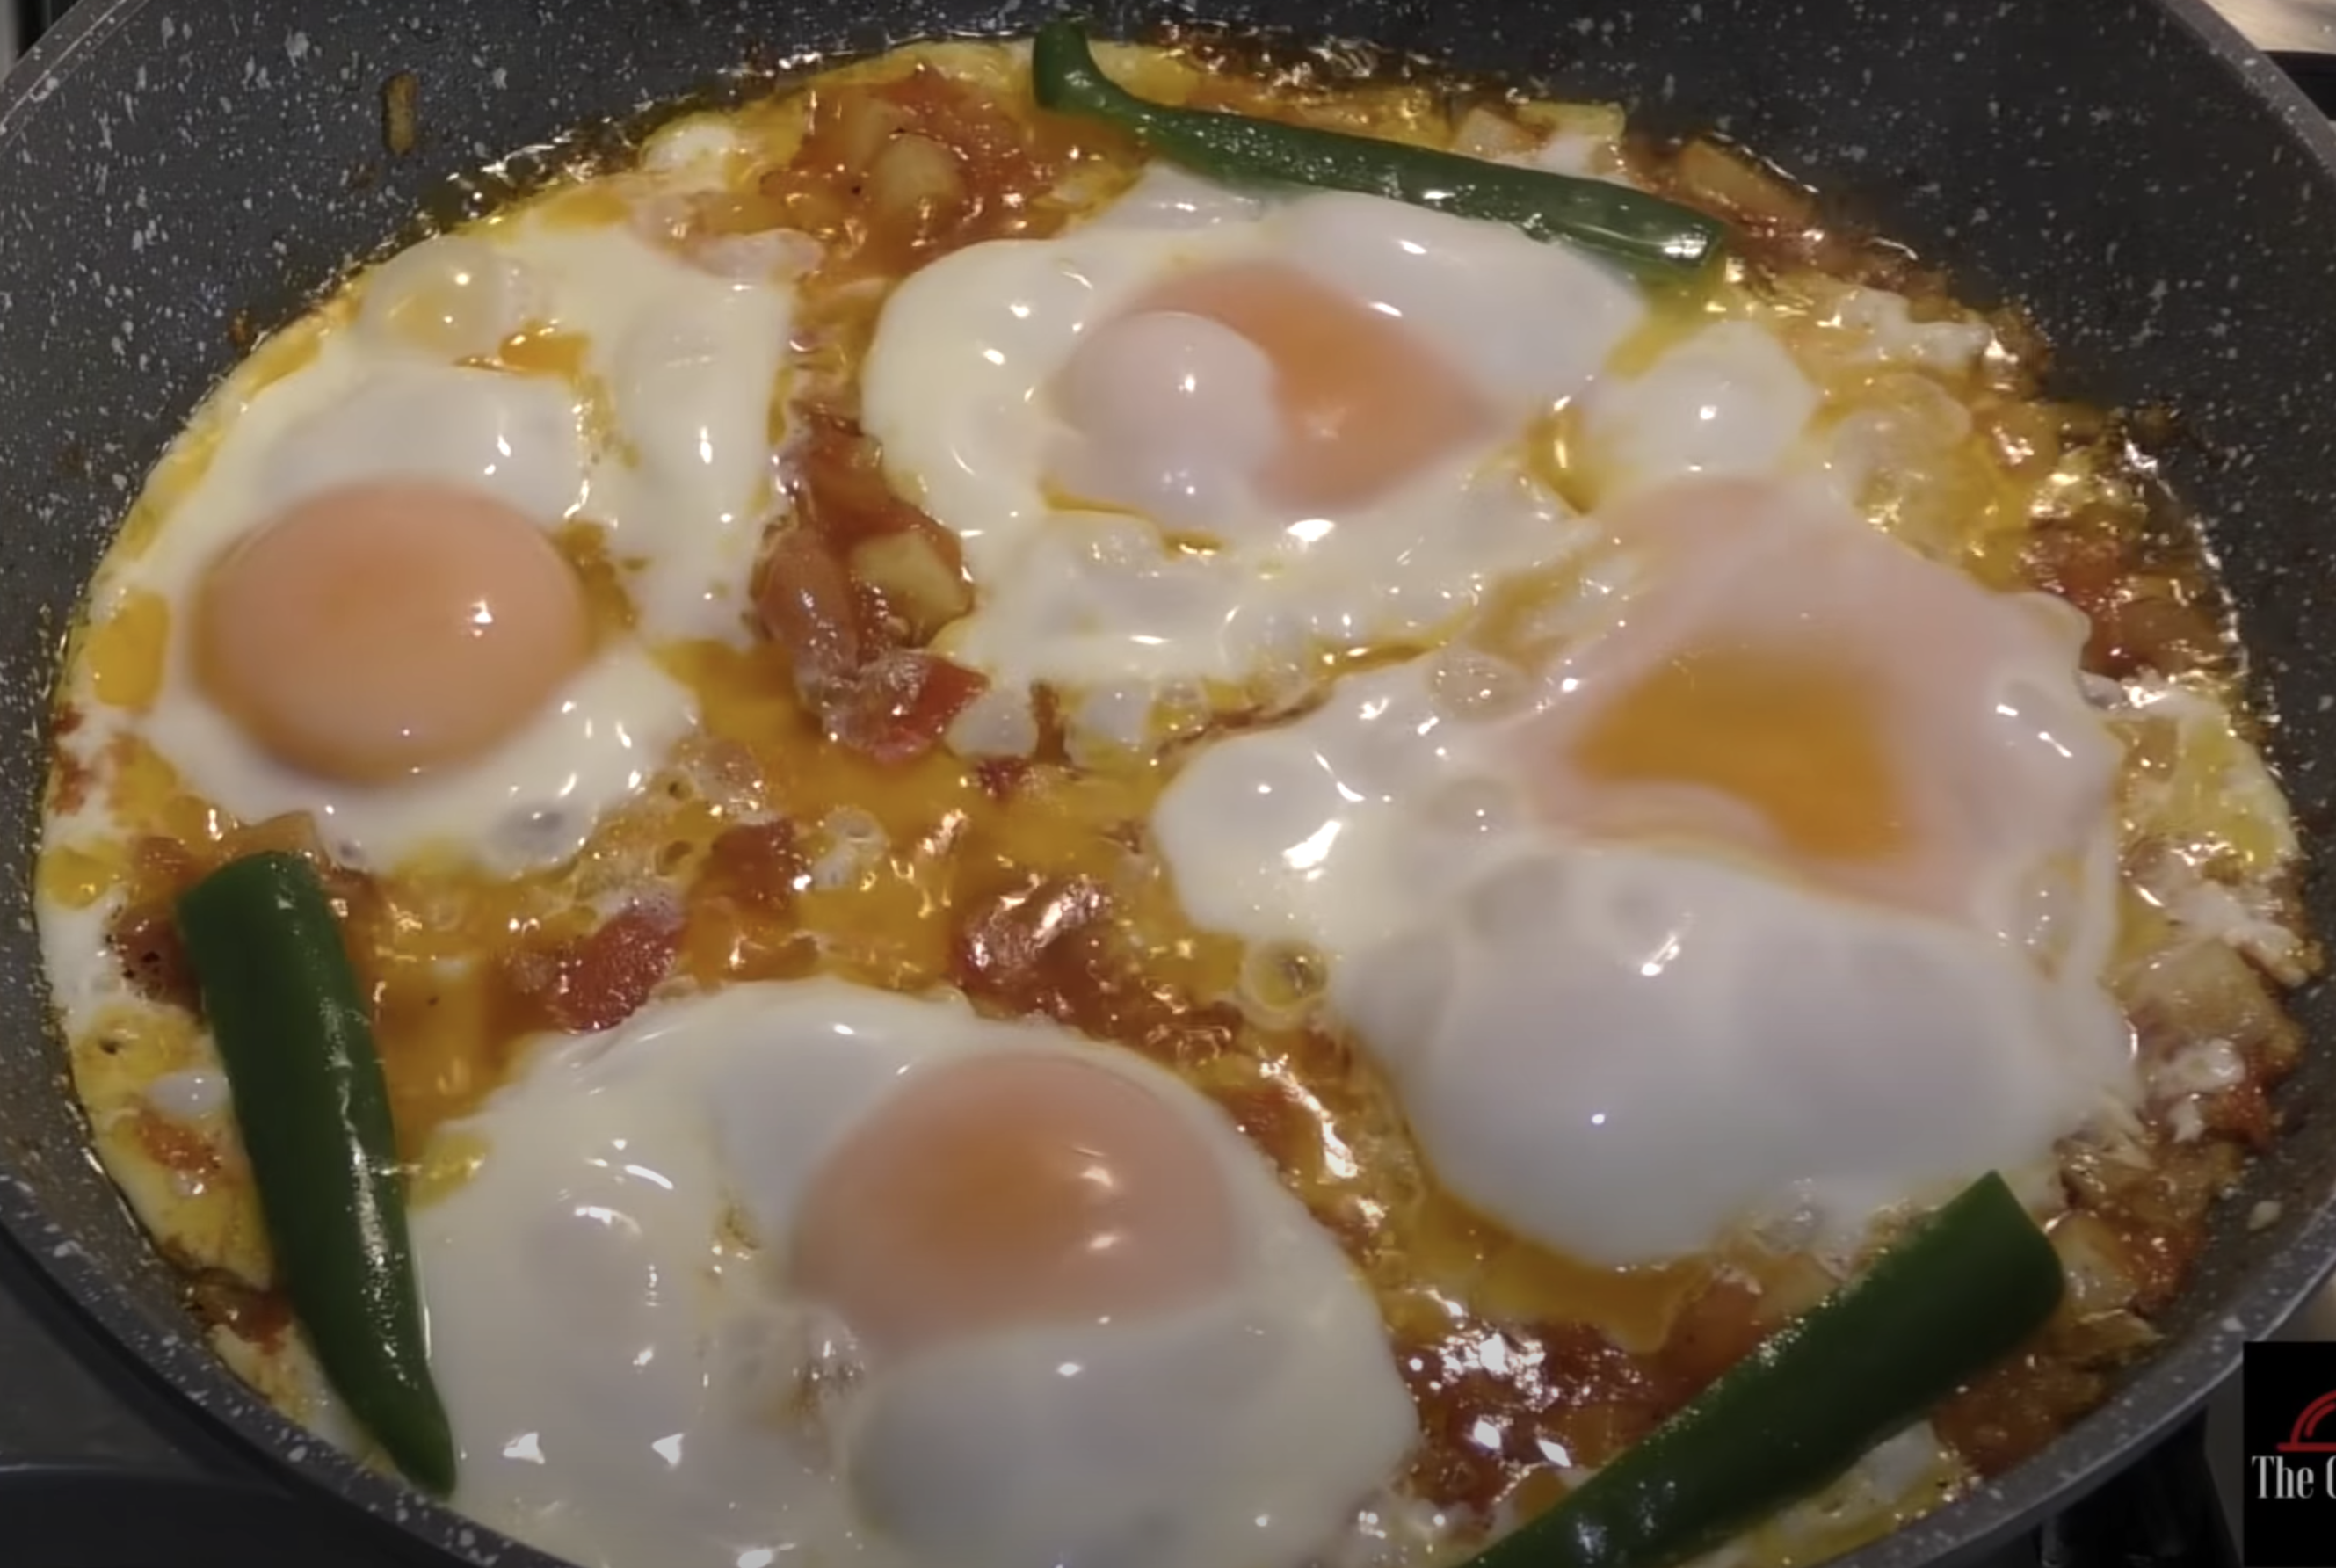
\includegraphics[width=0.30\textwidth]{recipePictures/EggTomatoPotatoAfghaniOmelette}
%\end{center}
%
%\begin{method}%[Preheat the oven to Gas Mark 4, Electric \temp{180}, Fan \temp{160}.]
%	...
%\end{method}

\end{document}